\section{策略模式}

\subsection{策略模式的引入}

\subsubsection{从模拟鸭子应用开始}
在模拟鸭子SimUDuck游戏中会出现各种鸭子,一边游泳戏水,一边呱呱叫。此系统的内部设计使用了标准的OO技术,设计了一个鸭子超类,并让各种鸭子继承此超类。
\begin{figure}[H]
    \vspace{-0.5em}
	\centering
	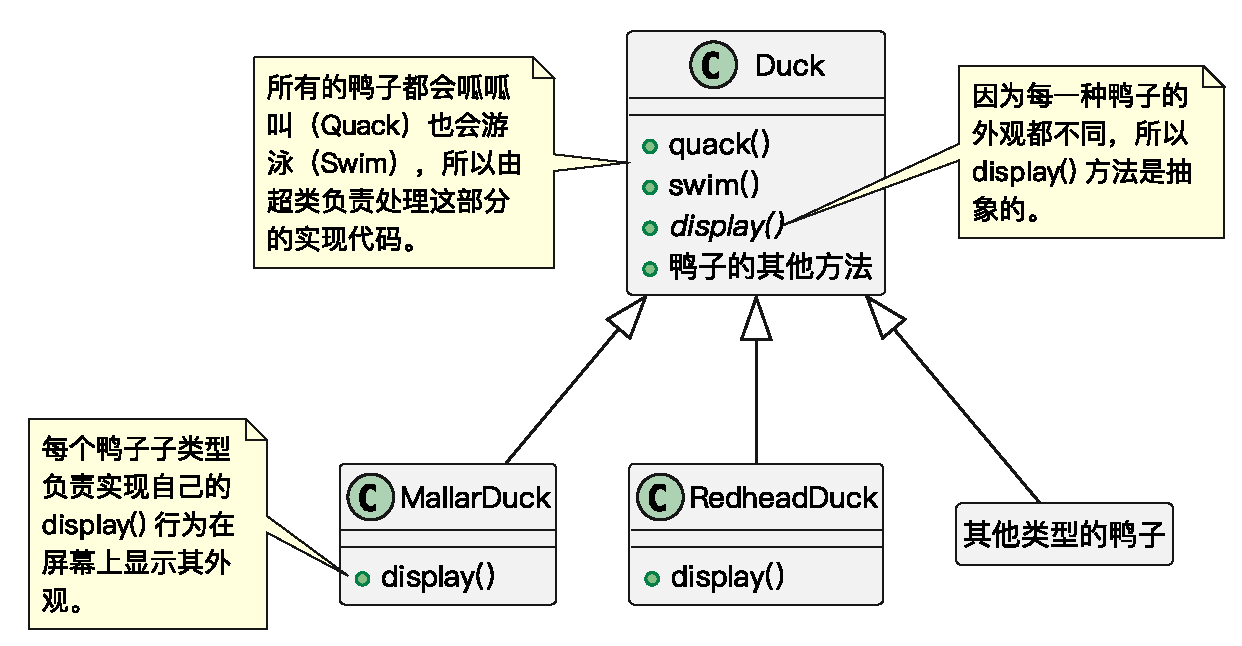
\includegraphics[width=0.75\textwidth]{images/SimUDuck1.eps}
    \vspace{-1em}
\end{figure}

现在需要添加功能使得鸭子可以飞。简单地修改鸭子父类,我们可以发现这样子橡皮鸭也可以飞,显然不是我们想要的。
\begin{itemize}
    \item 我们总是可以像使用\;\verb|quack()|\;方法一样在橡皮鸭中覆盖\;\verb|fly()|\;方法……
    \item 但是,当我们在程序中添加木制诱饵鸭子时会发生什么呢?他们不应该飞或嘎嘎……
    \item 高管们希望每六个月更新一次产品。每次更新中都会有新的\;\verb|Duck|\;子类,真是一场噩梦!
\end{itemize}

\begin{figure}[H]
    \vspace{-0.5em}
	\centering
	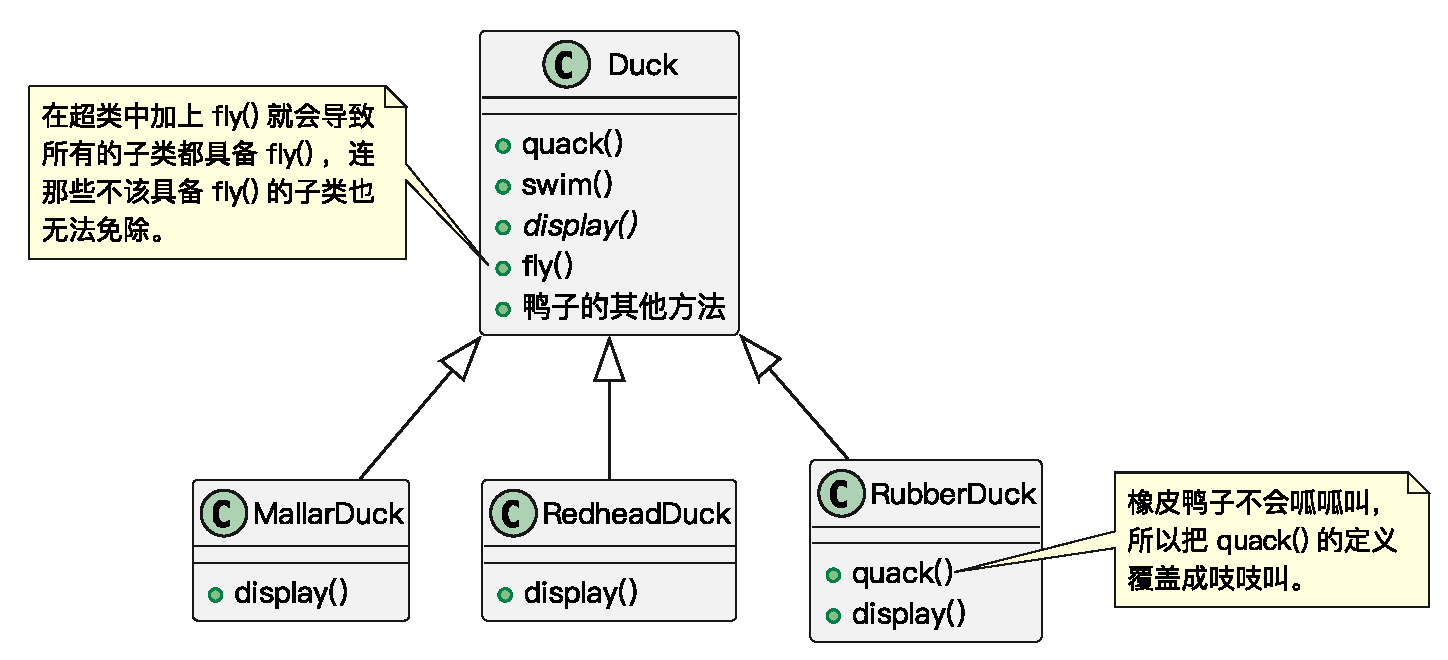
\includegraphics[width=0.75\textwidth]{images/SimUDuck2.eps}
    \vspace{-1em}
\end{figure}

我们知道,并非所有的子类都具有飞行和呱呱叫的行为,所以继承并不是适当的解决方式。那么使用接口会如何呢?

虽然\;\verb|Flyable|\;与\;\verb|Quackable|\;可以解決一部分问题(不会再有会飞的橡皮鸭),但是Java接口不具有实现代码,所以继承接口无法达到代码的复用,这意味着无论何时你需要修改某个行为,你必须得往下追踪并在每一个定义此行为的类中修改它,一不小心,可能会造成新的错误!这只能算是从一个恶梦跳进另一个恶梦。甚至,在会飞的鸭子中,飞行的动作可能还有多种变化……

\begin{figure}[H]
    \vspace{-0.5em}
	\centering
	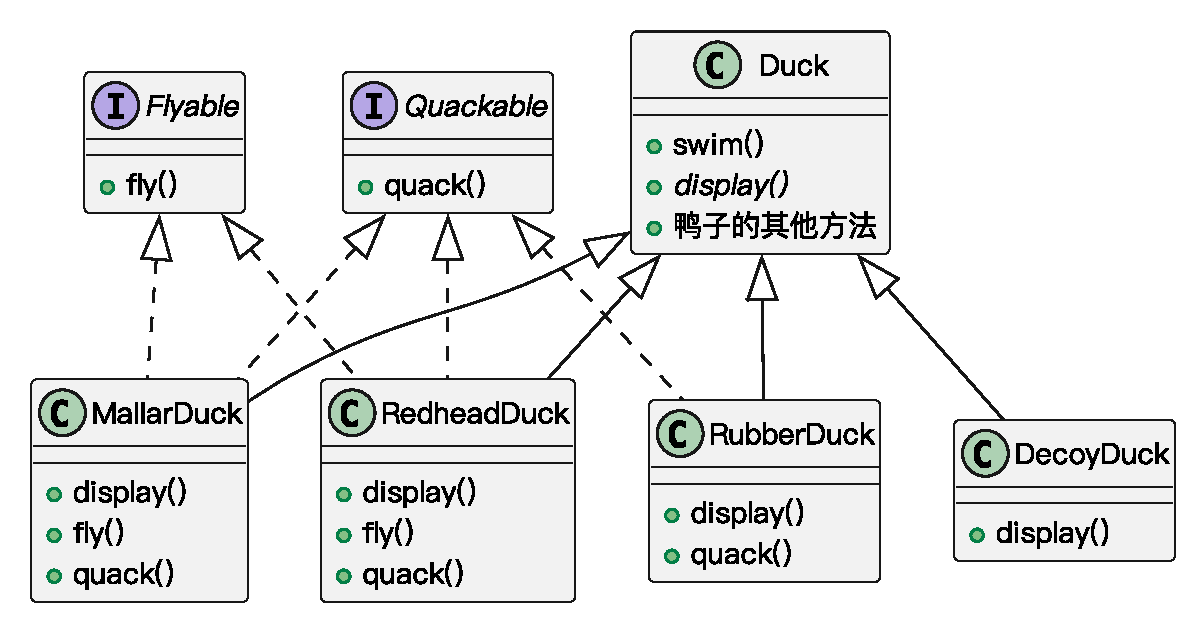
\includegraphics[width=0.75\textwidth]{images/SimUDuck3.eps}
    \vspace{-1em}
\end{figure}

\subsubsection{分开变化和不变的部分}
我们知道\;\verb|Duck|\;类内的\;\verb|fly()|\;和\;\verb|quack()|\;会随着鸭子的不同而改变。为了要把这两个行为从\;\verb|Duck|\;类中分开,我们将把它们从\;\verb|Duck|\;类中取出来,建立一组新类来代表每个行为。
\begin{figure}[H]
    \vspace{-0.5em}
	\centering
	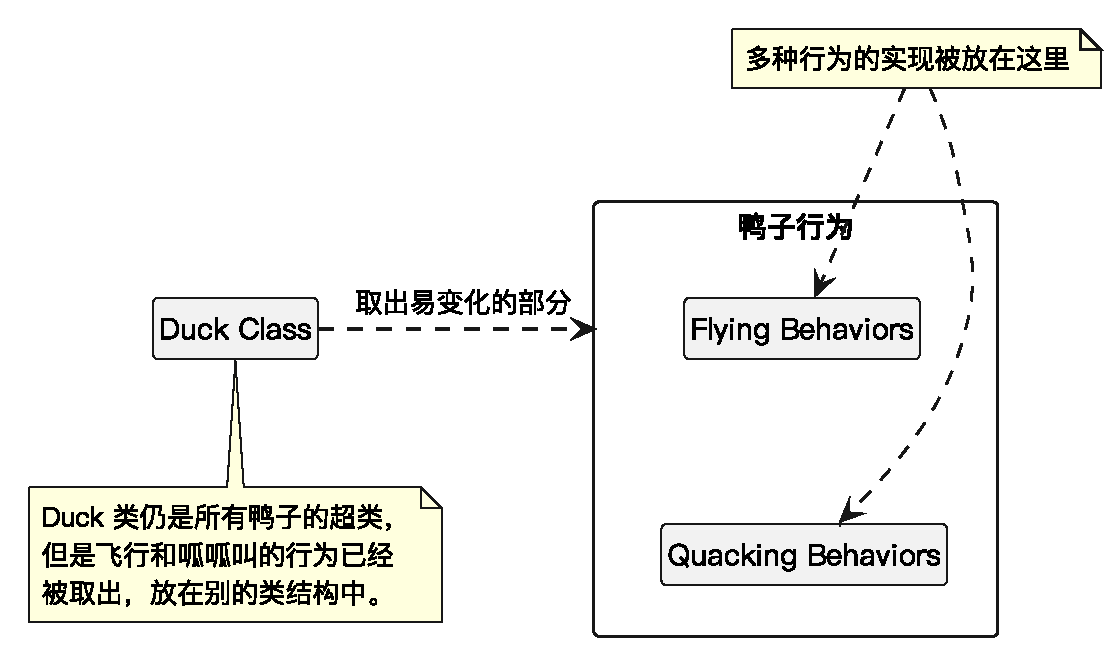
\includegraphics[width=0.65\textwidth]{images/SimUDuck4.eps}
    \vspace{-1em}
\end{figure}

\subsubsection{面向接口编程,而不是面向实现编程}
下图所示的设计,可以让飞行和呱呱叫的动作被其他的对象复用,因为这些行为已经与鸭子类无关了。而且我们可以新增一些行为,不会影响到既有的行为类,也不会影响使用到飞行行为的鸭子类。这样一来,有了继承的复用好处,却没有继承所带来的包袱。
\begin{figure}[H]
    \vspace{-0.5em}
	\centering
	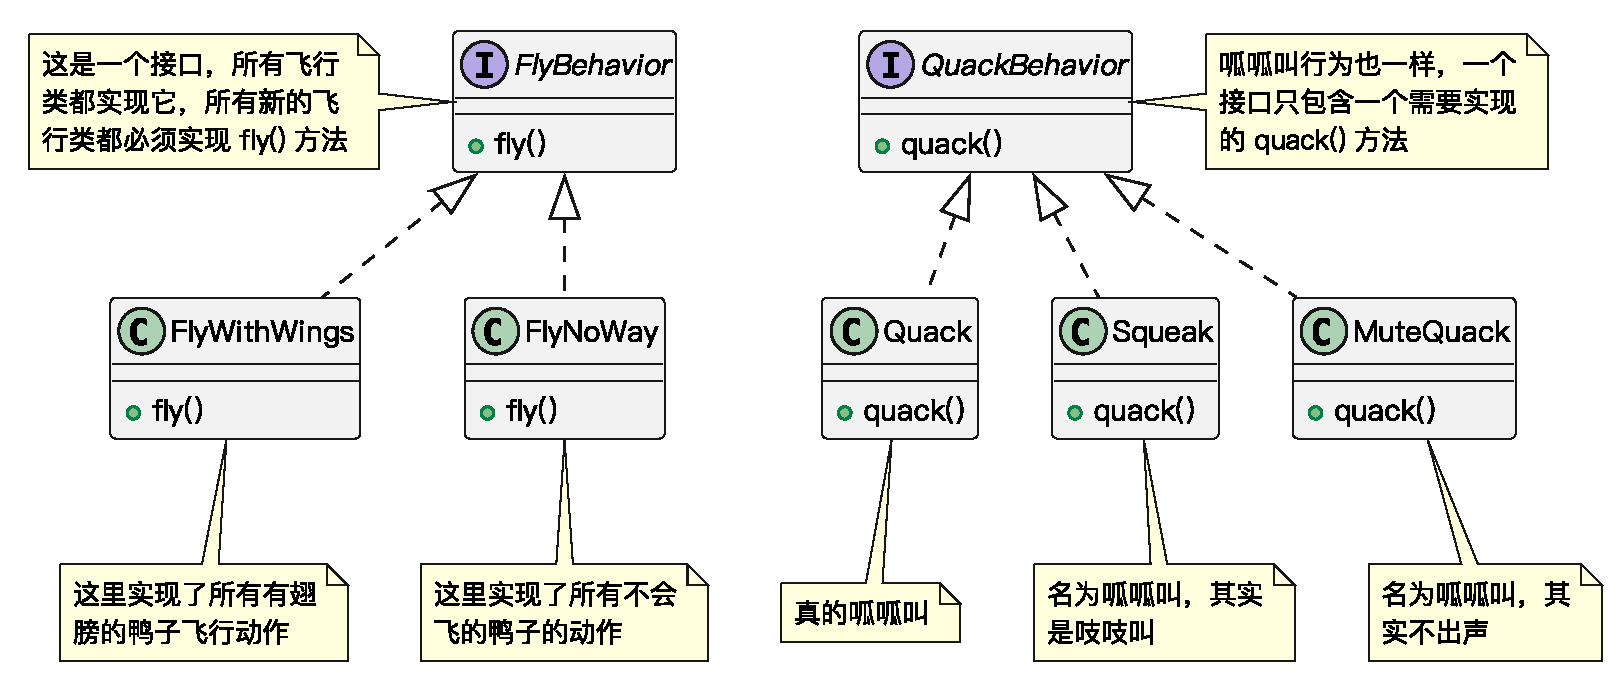
\includegraphics[width=0.9\textwidth]{images/SimUDuck5.eps}
    \vspace{-1em}
\end{figure}

\subsubsection{整合鸭子行为}
\begin{figure}[H]
    \vspace{-0.5em}
	\centering
	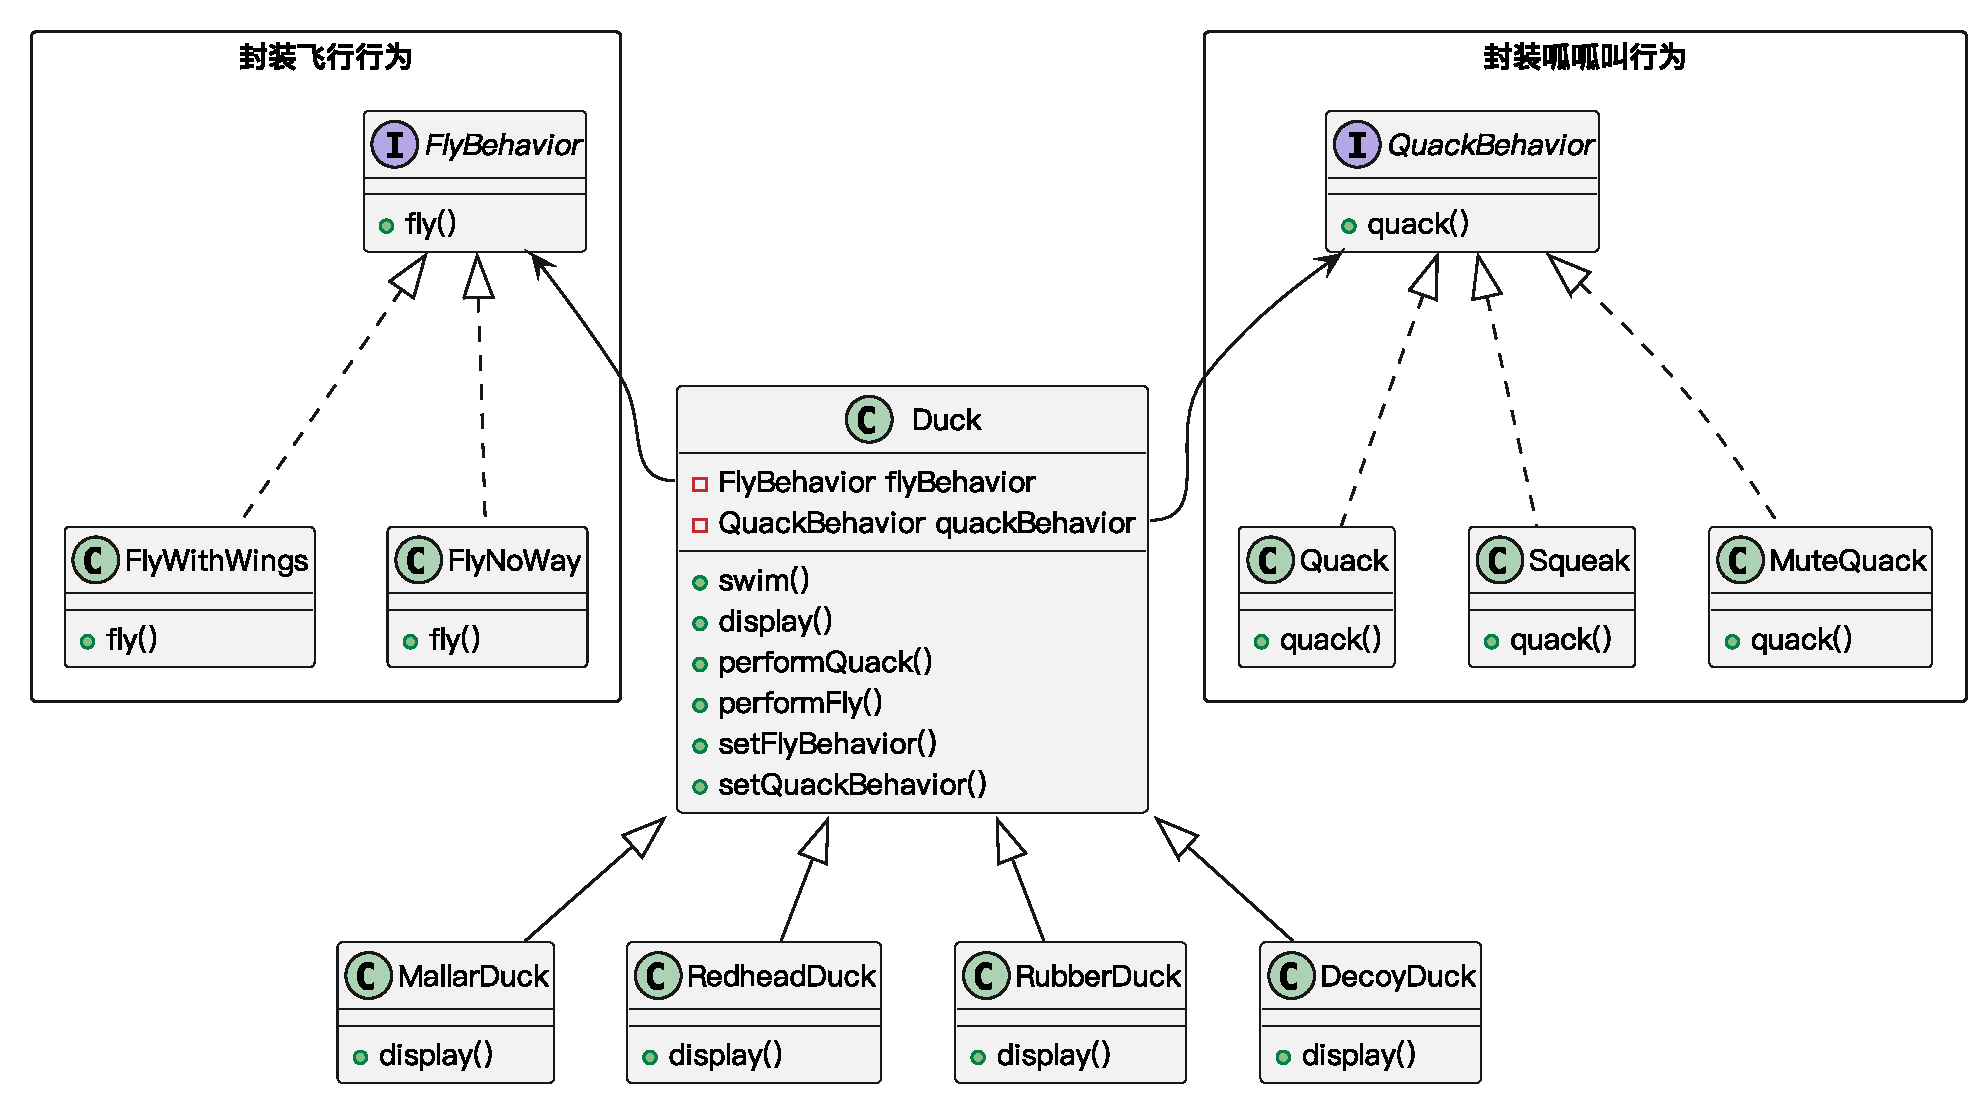
\includegraphics[width=0.95\textwidth]{images/SimUDuck6.eps}
    \vspace{-1em}
\end{figure}


\subsection{第一个设计模式:策略模式}
策略模式(Strategy Pattern)定义了一系列算法,分别封装起来,并使它们可替换。此模式让算法的变化独立于使用算法的客户。

\subsubsection{策略模式使用实例}
将文本流分成几行。由于存在许多用于将文本流分成行的算法,将所有这样的算法硬连接到类中是不可取的。
\begin{figure}[H]
    \vspace{-0.5em}
	\centering
	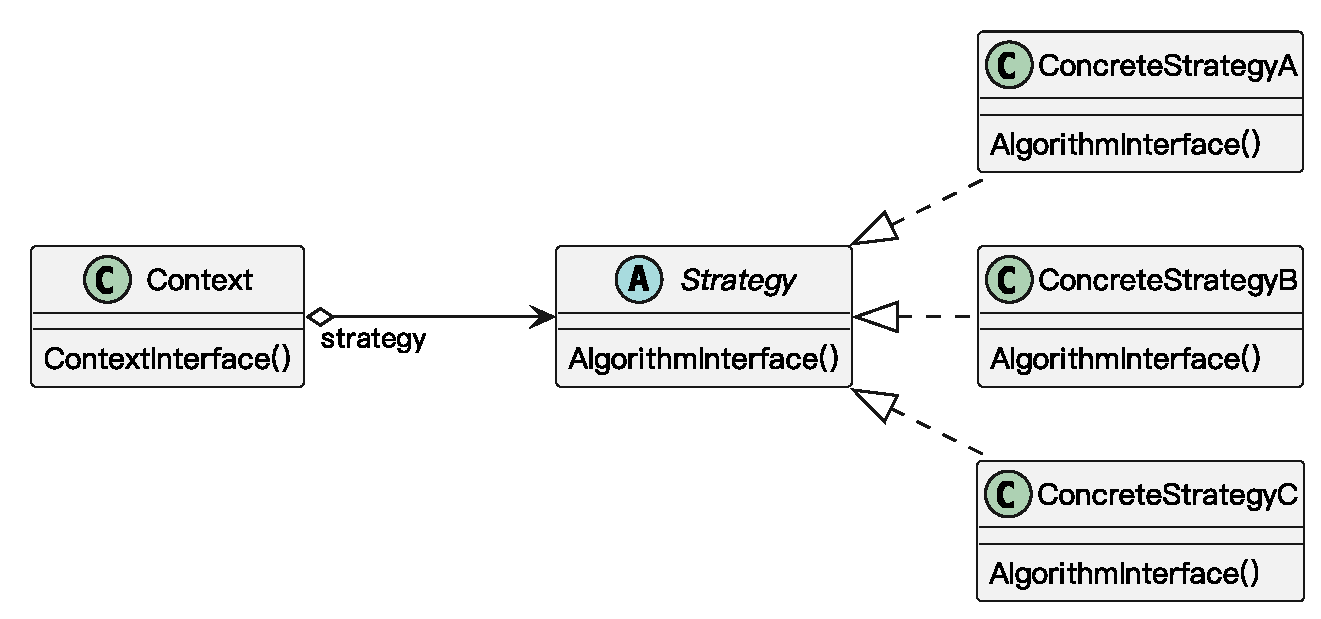
\includegraphics[width=0.58\textwidth]{images/策略模式.eps}
    \vspace{-1em}
\end{figure}


\begin{lstlisting}
public class Context{
    public void algorithm(String type){
        if(type.equals("strategyA")) {
            this.strategy = new ConcreteStrategyA();
        } else if(type.equals("strategyB")) {
            this.strategy = new ConcreteStrategyB();
        } else if(type.equals("strategyC")) {
            this.strategy = new ConcreteStrategyC();
        }
    }
}
\end{lstlisting}

\subsubsection{策略模式的使用场景}
\begin{itemize}
    \item 许多相关的类仅在\textbf{行为}上有所不同,策略提供了一种使用多种行为之一配置类的方法
    \item 需要\textbf{算法的不同变体}。例如,您定义了反映不同空间/时间权衡的算法,将这些变体实现为算法的类层次结构时,可以使用策略。
    \item 一种算法使用客户端不应该知道的数据。使用策略模式\textbf{可避免暴露复杂的、特定于算法的数据结构}。
    \item 一个类定义了许多行为,这些行为在其操作中显示为多个条件语句。此时可以代替这些条件,将相关的条件分支移到他们自己的\textbf{策略类}中。
\end{itemize}

\subsubsection{策略模式使用的结果}
\begin{itemize}
    \item 定义了相关算法家族。策略类的层次结构定义了一系列算法或行为,以供上下文重用。继承可以帮助排除算法的通用功能。
    \item 子类化的替代方法。
    \item 策略消除条件语句。
    \item 多种实现方式。策略可以提供相同行为的不同实现。客户可以选择具有不同时间和空间权衡的策略。
    \item 客户必须意识到不同的策略。这种模式有一个潜在的缺点,即\textbf{客户在选择合适的策略之前必须先了解策略的不同},不然客户可能会遇到实现问题。
    \item 策略和上下文之间的通信开销。
    \item 对象数量增加。
    \item  模式一般都会有的缺点:
    \begin{itemize}
        \item 增加设计的复杂度和增加类的个数(增加辅助类)
        \item 增加隔阂和方法调用,降低软件运行的效率,但是已经不是目前主要的问题
    \end{itemize}
    \item Java的加密方法、时间显示算法等都是通过策略模式实现的。
\end{itemize}